\chapter{Implementacja systemu}

\section{Backend - API do zarządzania systemem}

\subsection{Struktura API i kluczowe endpointy}
\begin{figure}[H]
  \centering
  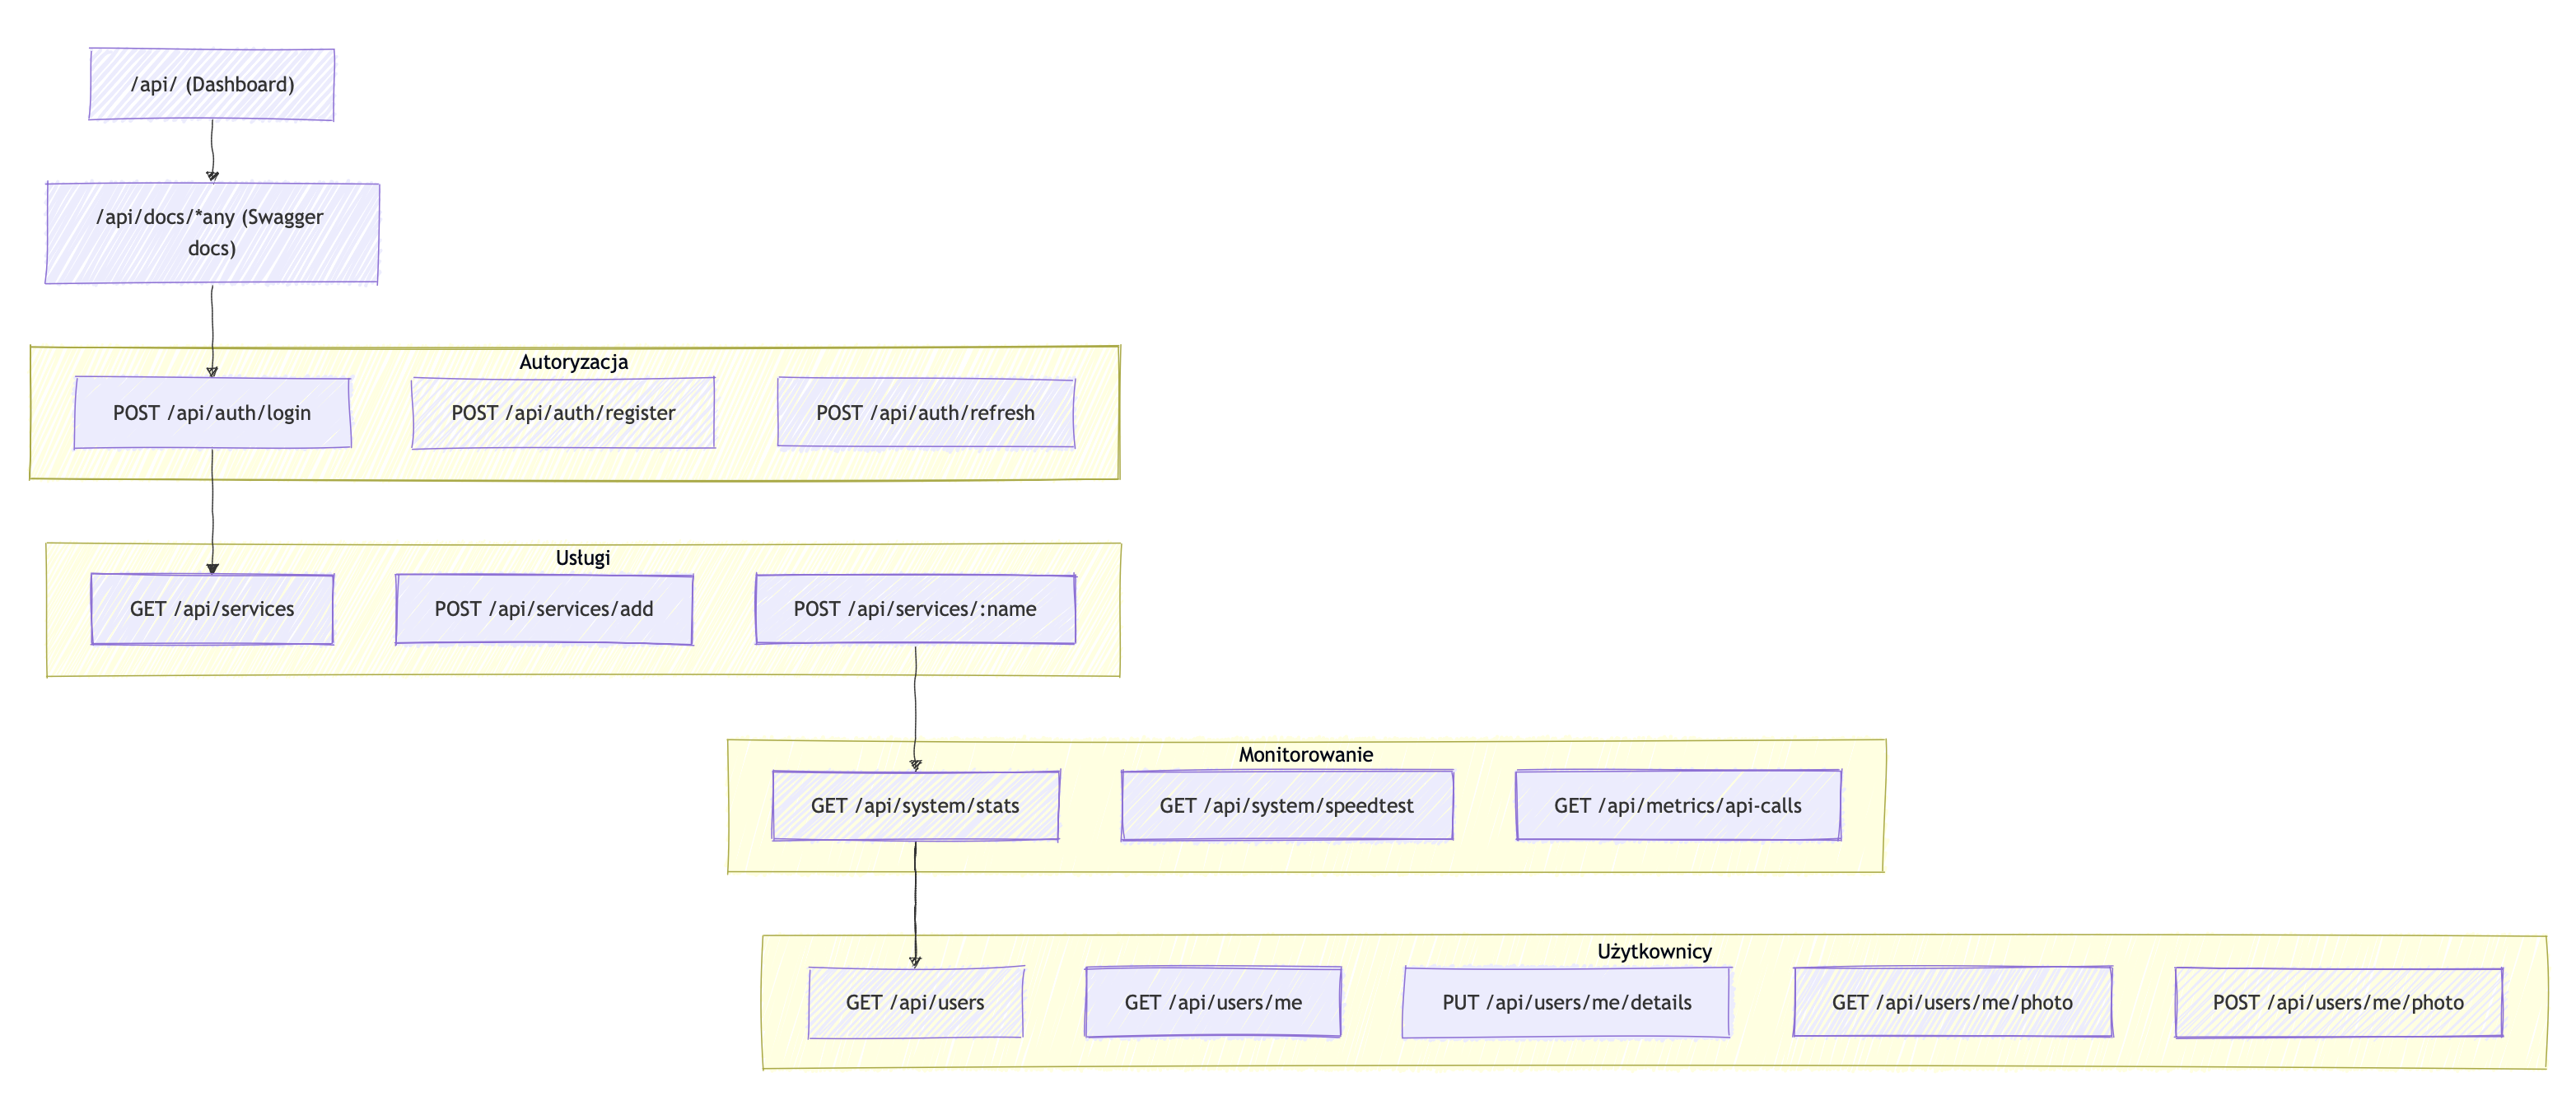
\includegraphics[width=1\textwidth]{./chapters/mermeid/schemat api.png}
  \caption{Schemat architektury API aplikacji HomeNest.}
  \label{fig:api_schema}
\end{figure}
System został zaprojektowany jako aplikacja webowa z backendem opartym na języku Go, wykorzystującym framework Gin, zapewniającym wysoką wydajność oraz możliwość łatwego definiowania tras i obsługi żądań HTTP. API udostępnia szereg endpointów pozwalających na zarządzanie użytkownikami, usługami, monitorowanie systemu oraz uwierzytelnianie.

\subsubsection{Autoryzacja i uwierzytelnianie}
\begin{itemize}
    \item \textbf{POST /api/auth/login} - logowanie użytkownika i zwrócenie tokena JWT,
    \item \textbf{POST /api/auth/register} - rejestracja nowego użytkownika,
    \item \textbf{POST /api/auth/refresh} - odświeżenie tokena JWT.
\end{itemize}

\subsubsection{Zarządzanie usługami}
\begin{itemize}
    \item \textbf{GET /api/services} - pobranie listy aktualnie zarejestrowanych usług,
    \item \textbf{POST /api/services/add} - dodanie nowej usługi do systemu,
    \item \textbf{POST /api/services/:name} - przełączenie (uruchomienie/zatrzymanie) wybranej usługi według nazwy.
\end{itemize}

\subsubsection{Monitorowanie systemu}
\begin{itemize}
    \item \textbf{GET /api/system/stats} - pobranie statystyk systemowych, takich jak zużycie CPU, RAM, przestrzeń dyskowa,
    \item \textbf{GET /api/system/speedtest} - pobranie wyników testu prędkości połączenia internetowego,
    \item \textbf{GET /api/metrics/api-calls} - pobranie liczby zapytań API z ostatnich dni.
\end{itemize}

\subsubsection{Zarządzanie użytkownikami}
\begin{itemize}
    \item \textbf{GET /api/users} - lista użytkowników (dostępna tylko dla administratora),
    \item \textbf{GET /api/users/me} - pobranie danych zalogowanego użytkownika,
    \item \textbf{PUT /api/users/me/details} - aktualizacja danych zalogowanego użytkownika,
    \item \textbf{POST /api/users/me/photo} - przesłanie zdjęcia profilowego,
    \item \textbf{GET /api/users/me/photo} - pobranie zdjęcia profilowego użytkownika.
\end{itemize}

\subsubsection{Dashboard i dokumentacja}
\begin{itemize}
    \item \textbf{GET /api/} - główny endpoint dashboardu aplikacji,
    \item \textbf{GET /api/docs/*any} - dokumentacja API generowana automatycznie przy użyciu narzędzia Swagger.
\end{itemize}

\subsubsection{Podsumowanie}
Zaprojektowane API jest modularne, bezpieczne i łatwe do rozszerzenia. Struktura endpointów została opracowana w sposób zgodny z dobrymi praktykami REST, umożliwiając wygodne zarządzanie zasobami systemowymi i użytkownikami, a dzięki wykorzystaniu frameworka Gin osiągnięto wysoką wydajność obsługi żądań. Endpointy są chronione przez mechanizmy JWT i w zależności od kontekstu użytkownika odpowiednio ograniczają dostęp do operacji administracyjnych.


\subsection{Obsługa uwierzytelniania i autoryzacji}

System uwierzytelniania i autoryzacji opiera się na tokenach JWT (JSON Web Token). Mechanizm ten zapewnia bezpieczną kontrolę dostępu do zasobów systemu, umożliwiając przypisanie użytkownikom odpowiednich ról i ograniczenie dostępu do krytycznych operacji administracyjnych.

\subsubsection{Proces uwierzytelniania}
Każdy użytkownik musi zalogować się do systemu, podając swoje dane uwierzytelniające. Po pomyślnej weryfikacji hasła system generuje token JWT, który służy do autoryzacji kolejnych żądań API. Token zawiera informacje o użytkowniku oraz jego roli w systemie.

Kluczowe endpointy:
\begin{itemize}
    \item \textbf{POST /api/register} - Rejestracja nowego użytkownika,
    \item \textbf{POST /api/login} - Logowanie użytkownika i zwrócenie tokena JWT.
\end{itemize}
\newpage
\section{Frontend - Interfejs uzytkownika}

\subsection{Projekt UI/UX}

Z założenia interfejs użytkownika powinien być jak najprostszy oraz jak najbardziej ułatwiać użytkownikowi korzystanie z systemu. Powininen on umożliwiać użytkownikowi korzystanie z systemu w sposób zamierzony oraz uniemożliwiać korzystanie z systemu w sposób niezgodny z przeznaczeniem.
\subsubsection{Założenia projektowe}
Podstawowe cele projektowe interfejsu obejmowały:
\begin{itemize}
    \item Czytelność i prostota obsługi,
    \item Spójność wizualną oraz intuicyjna nawigacja,
    \item Minimalizacja liczby kliknięć wymaganych do wykonania operacji,
    \item Odpowiednia organizacja informacji w oparciu o hierarchię wizualną.
\end{itemize}

\subsubsection{Struktura interfejsu}
Projekt składa się z kilku widoków które zostaną opisane poniżej:
\paragraph{Strona Główna} - Strona przedstawia statystyki wykorzystania systemu oraz podstawowe informacje dotyczące środowiska uruchomieniowego.
\begin{figure}[H]
  \centering
  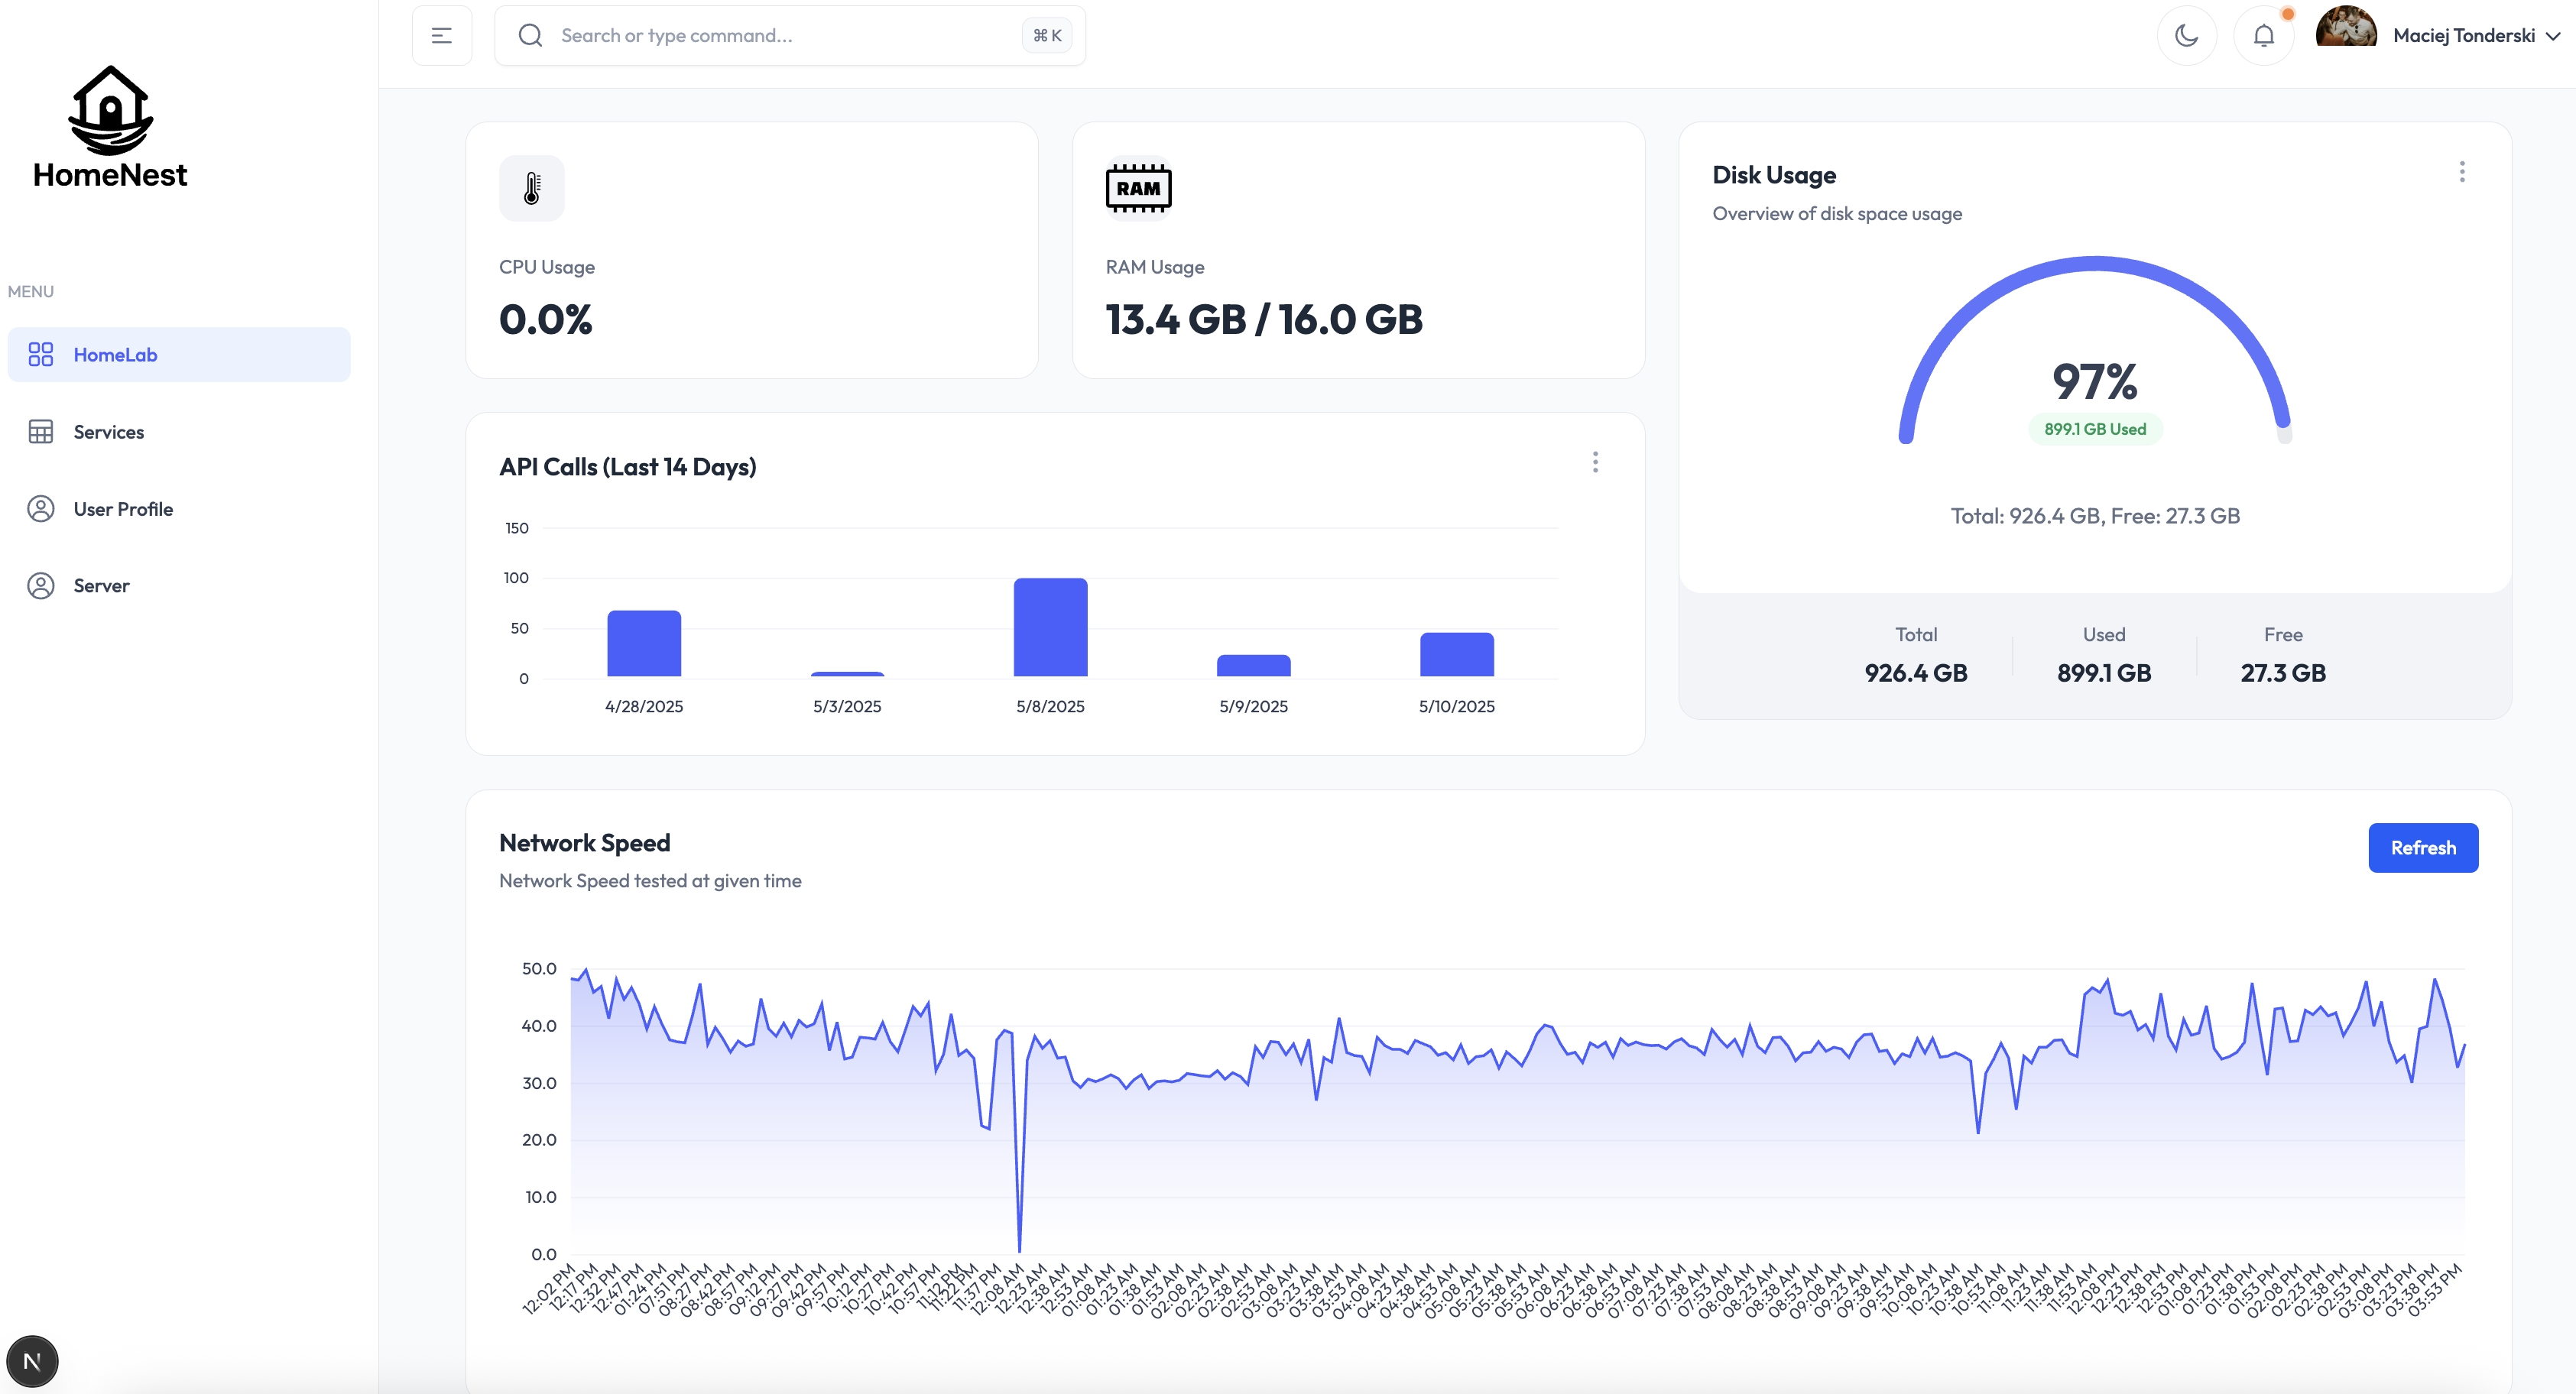
\includegraphics[width=1\textwidth]{./chapters/assets/UI_HomePage.png}
  \caption{Strona główna aplikacji Homelab.}
  \label{fig:ui_homepage}
\end{figure}
\begin{itemize}
    \item \textbf{Panel Informacyjny - wykorzystanie CPU} - Zawiera procentową wartość użycia procesora.
    \item \textbf{Panel Informacyjny - wykorzystanie RAM} - Zawiera informację ile GB pamięci RAM jest obecnie w użyciu oraz dostępną ilość pamięci RAM.
    \item \textbf{Wykres - Wykorzystanie Dysku} - Zawiera informację o wykorzystaniu dysku - ilość zajętej oraz dostępnej przestrzeni dyskowej.
    \item \textbf{Wykres - Ilość zapytań API apilikacji w ostatnich 14 dniach} - Pokazuje ile zapytań do aplikacji API zostało wykonanych w ostatnich 14 danich. Jeżeli aplikacja nie wykonywała zapytań do bazy przez ostatnie 14 dni codziennie umieszczne jest ostatnie 14 wpisów z bazy danych.
    \item \textbf{Wykres - Prędkość internetu} - System zgodnie z harmonogramem sprawdza prędkość podłączonego łącza internetowego i wyświetla je w formie tabeli w tym miejscu.
\end{itemize}

\paragraph{Strona Logowania oraz Rejestracji} - Strona umożliwa użytkownikowi wprowadzenie danych niezbęnych do umożliwienia korzystania z systemu. Użytkownik może się zalogować lub zarejestrować.
\begin{figure}[H]
  \centering
  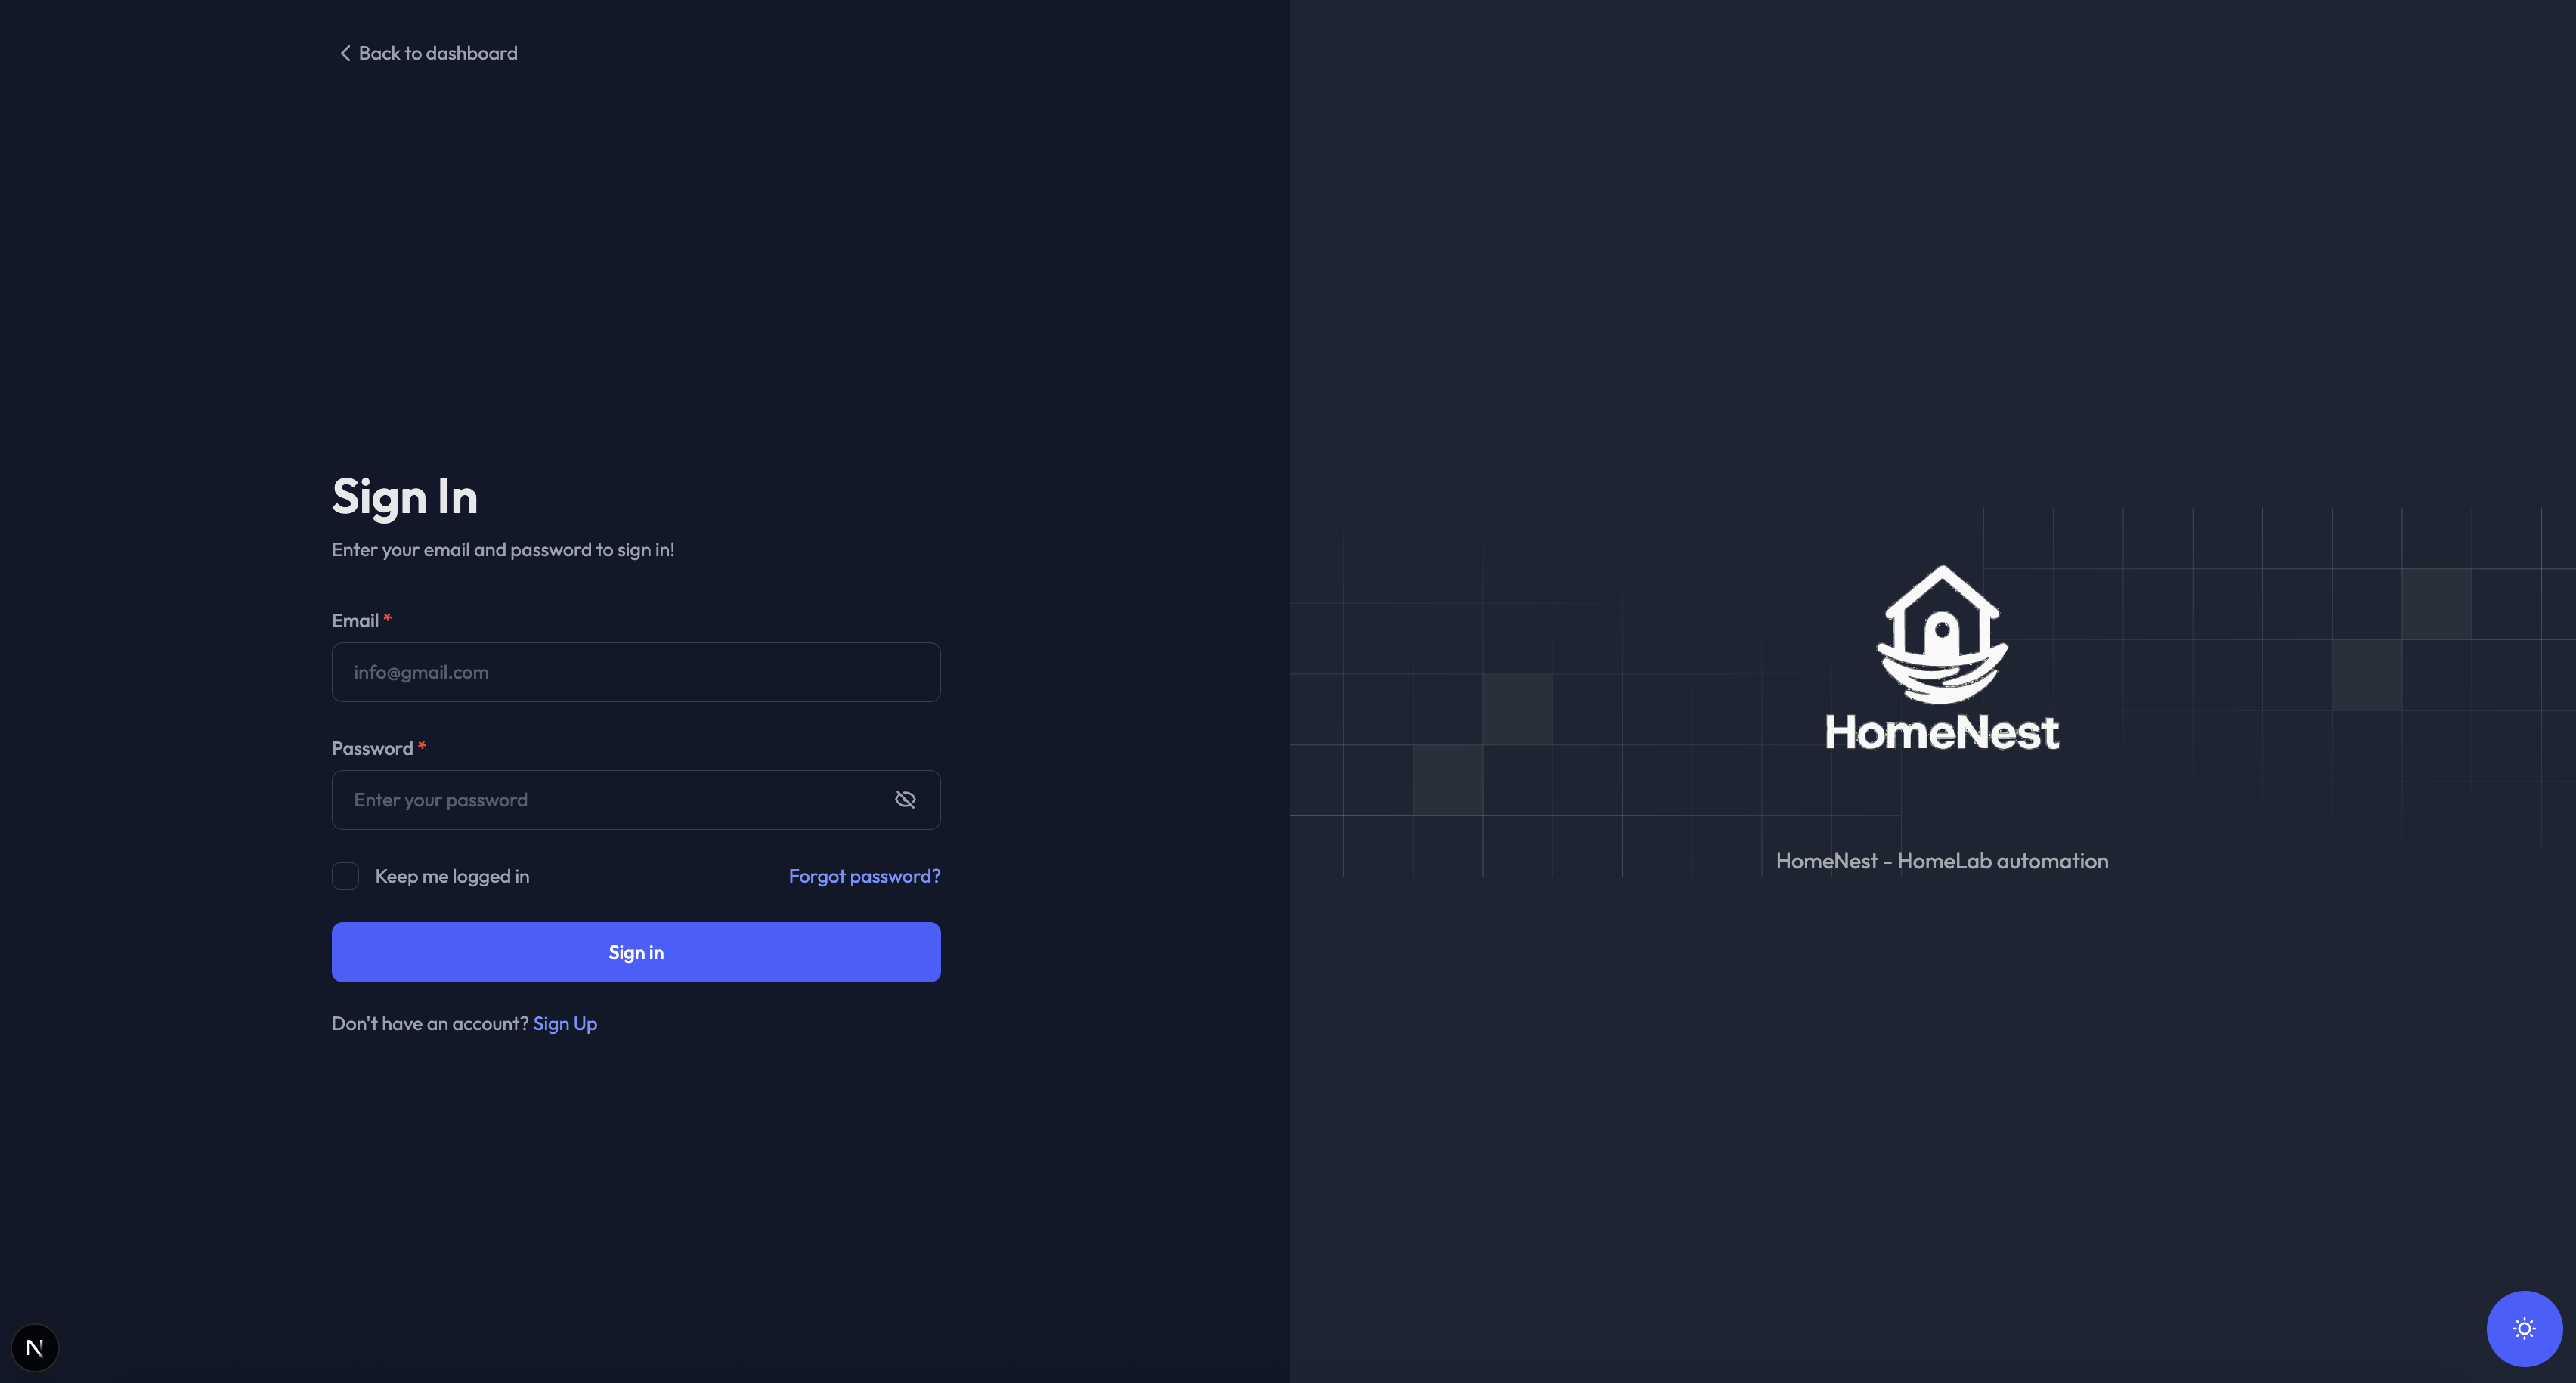
\includegraphics[width=1\textwidth]{./chapters/assets/login_page.png}
  \caption{Strona logowania do serwisu wyświetlająca logo oraz pola do wprowadzenia danych logowania}
  \label{fig:ui_login}
\end{figure}

\begin{figure}[H]
  \centering
  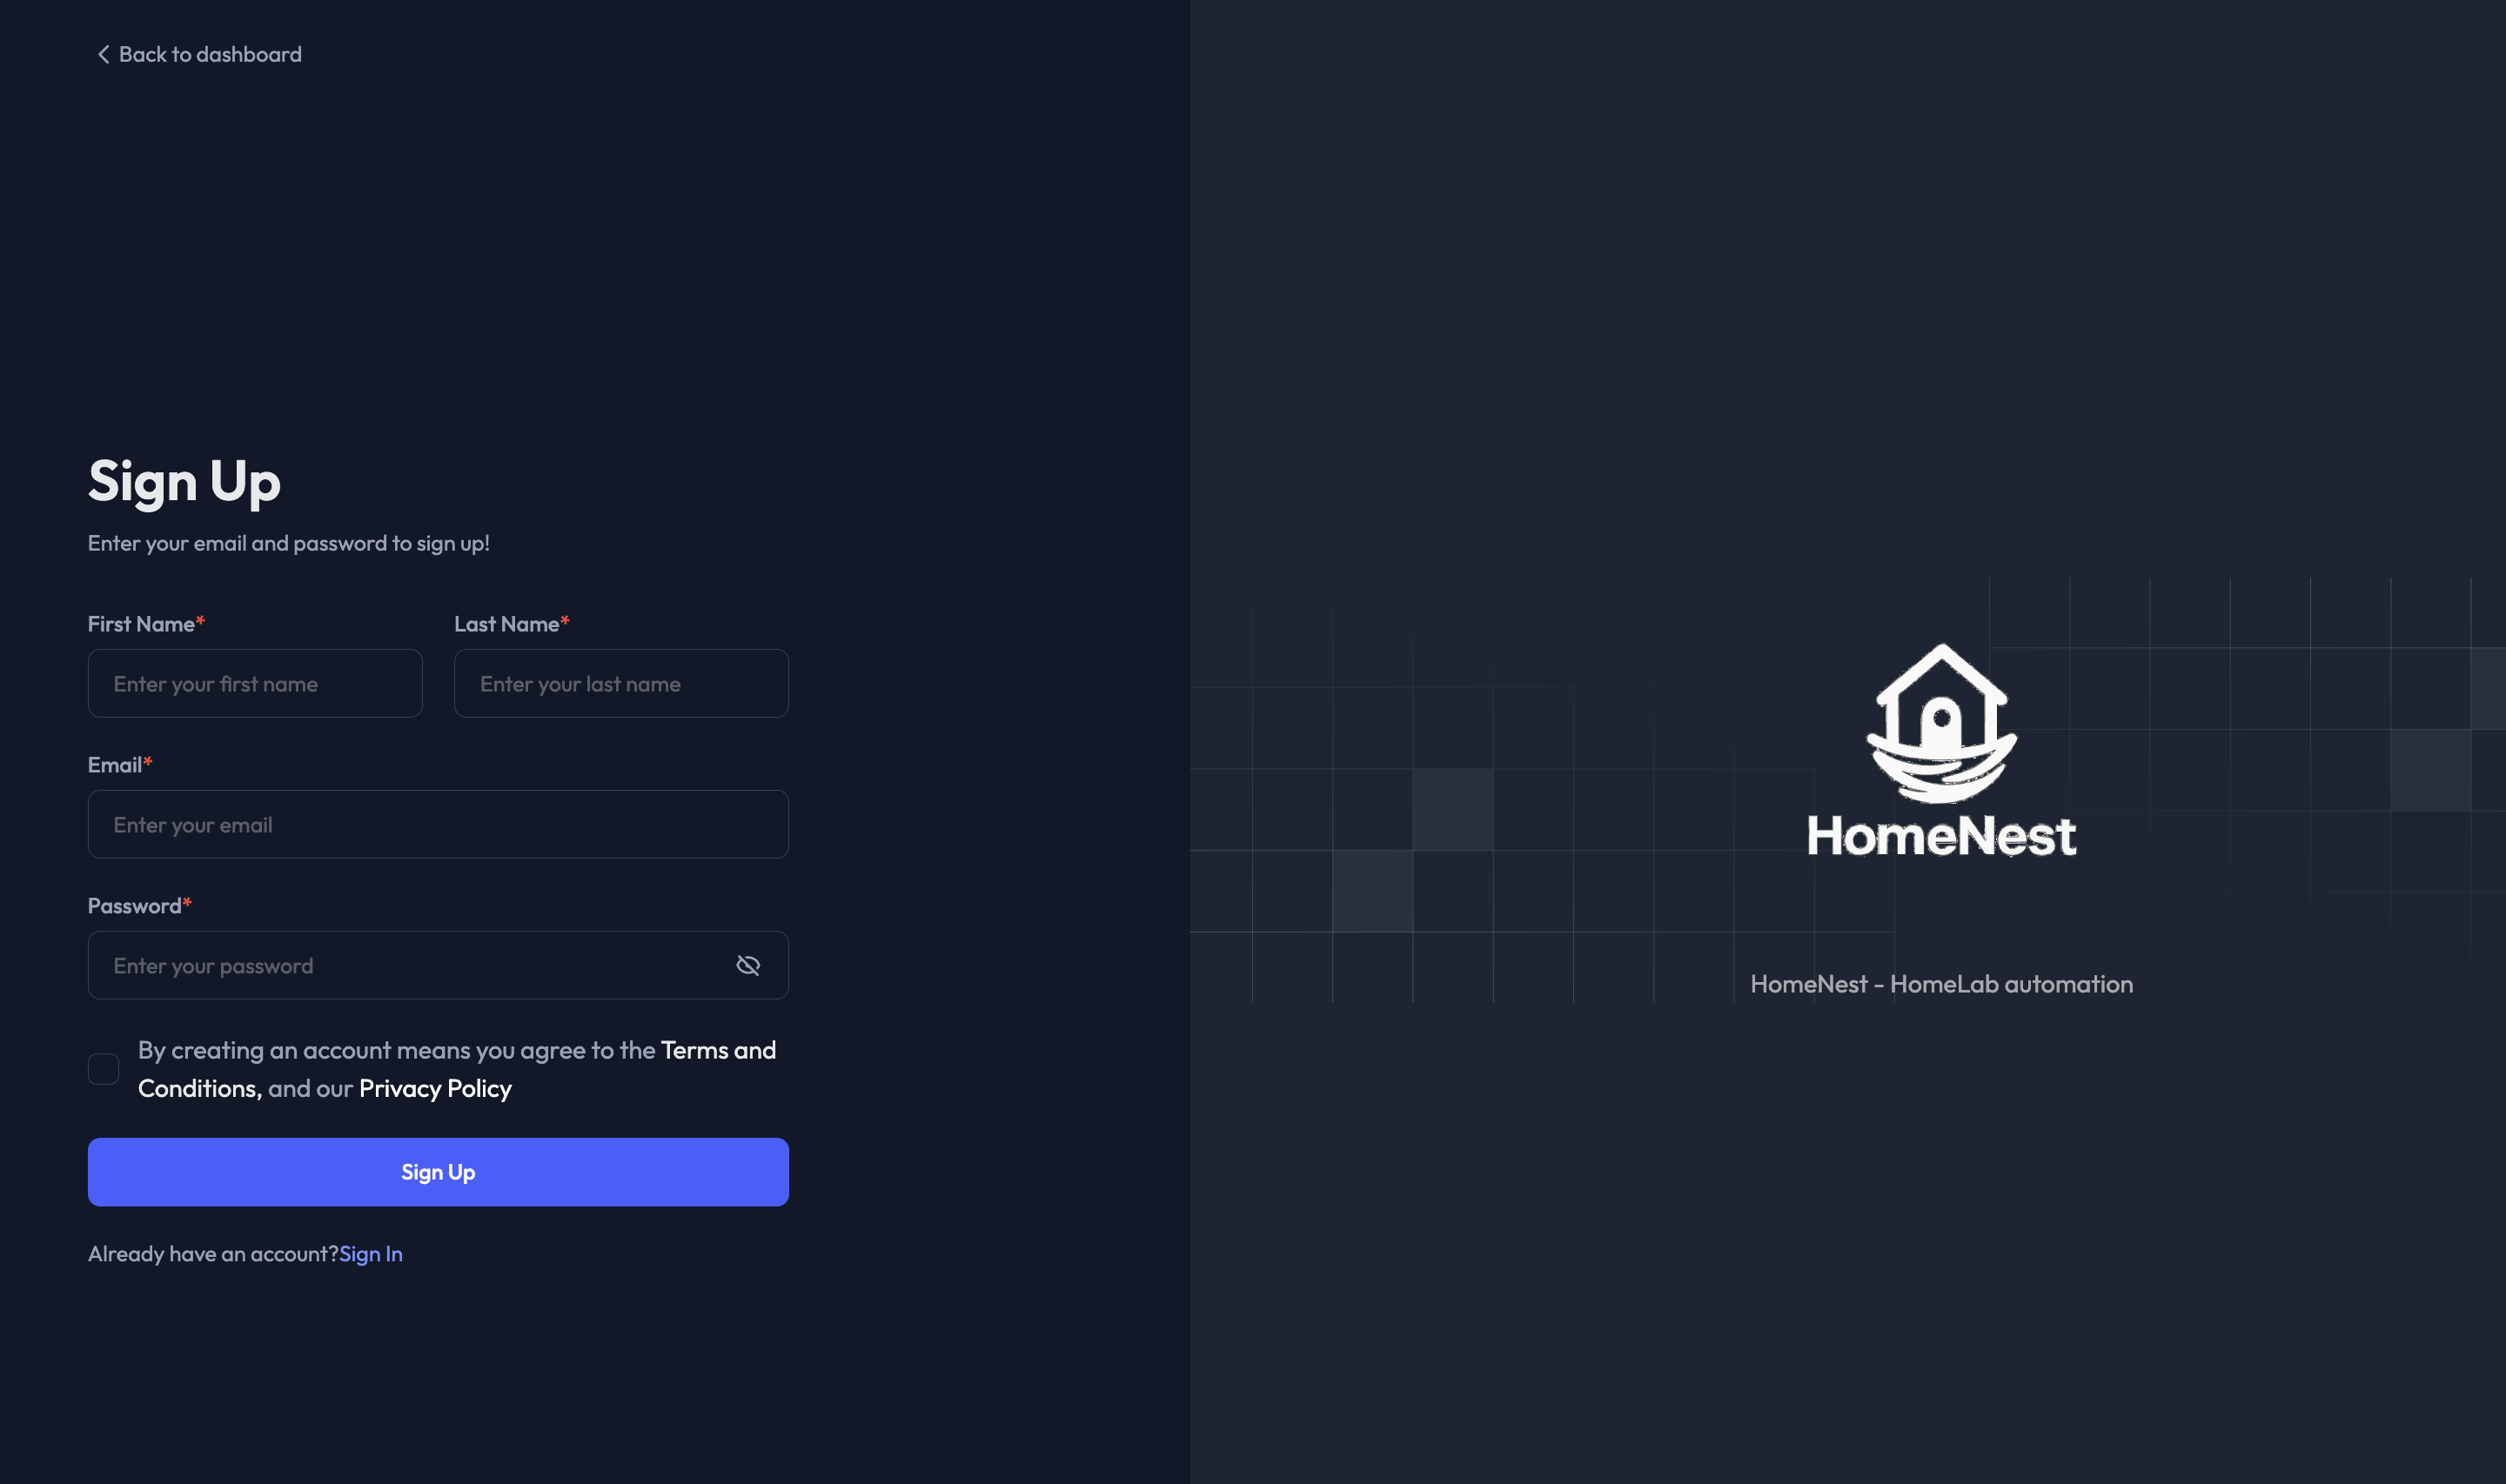
\includegraphics[width=1\textwidth]{./chapters/assets/signup_page.png}
  \caption{Strona Rejestracji do serwisu wyświetlająca logo oraz pola do wprowadzenia danych rejestracji}
  \label{fig:ui_signup}
\end{figure}
Użytkownik może się w tym miejscu zalogować lub zarejestrować przy pomocy adresu email oraz hasła. Rejestracja wymaga podania również swojego imienia i nazwiska oraz zaakceptowania polityk korzystania z serwisu, które będą dodane w późniejszym etapie rozwoju aplikacji.
Możliwa jest również zmiana kolorystyki poprzez naciśnięcie przycisku w prawym dolnym rogu ekranu, co spowoduje zmianę motywu z jasnego na ciemny lub przeciwnie.

\paragraph{Strona przedstawienia oraz integracji Serwisów} - Strona pokazuje obecnie dodane serwisy dostępne w systemie. Umożliwia dodanie własnego serwisu, uruchomienie lub zatrzymanie go oraz przejście do strony HTTP serwisu.
\begin{figure}[H]
  \centering
  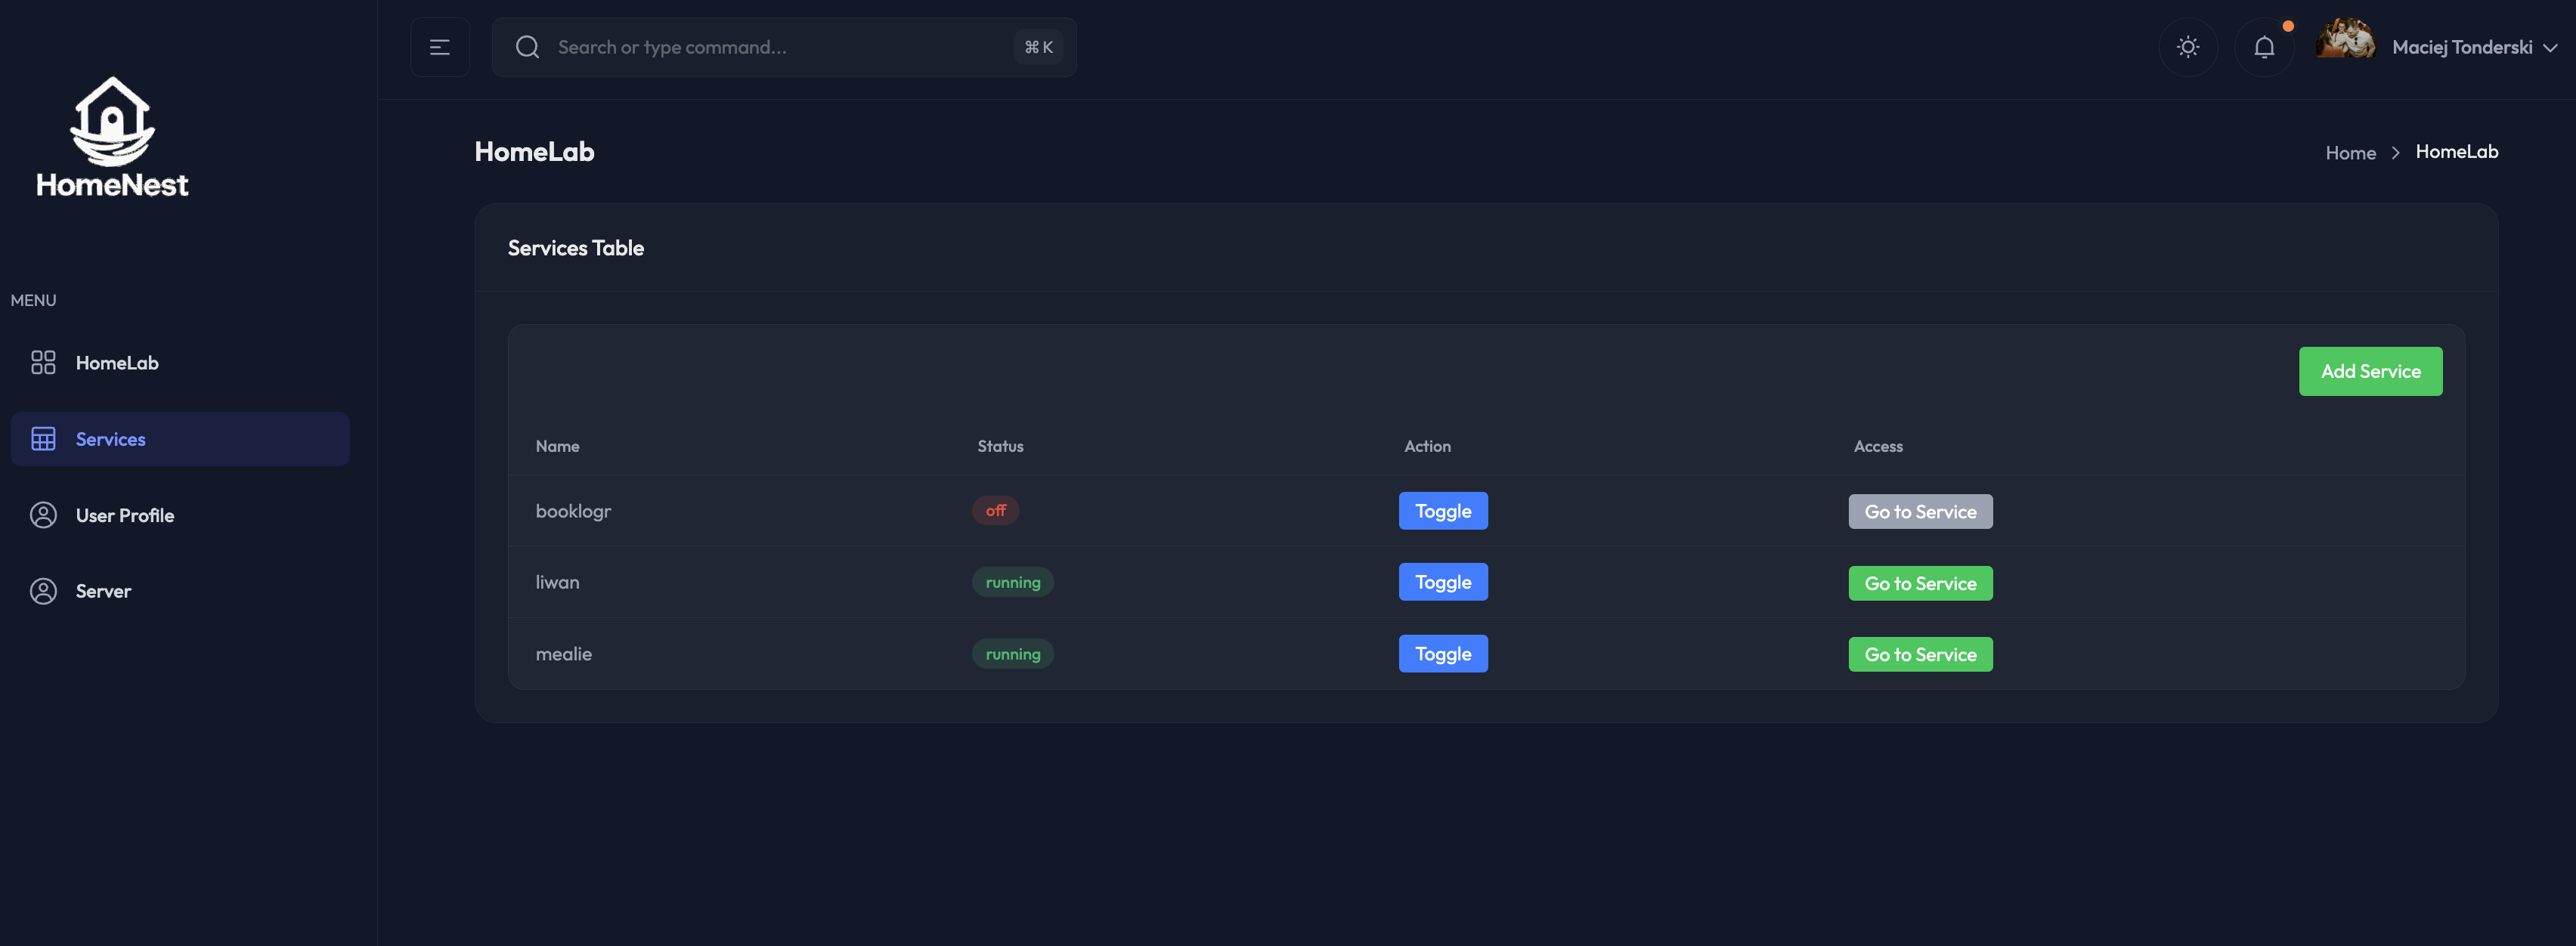
\includegraphics[width=1\textwidth]{./chapters/assets/services_page.png}
  \caption{Podstrona aplikacji odpowiedzialna za wyświetlanie stanu obecnie uruchomionych aplikacji, pozwalająca na ich zarządzanie oraz przekierowująca użytkownika do serwisu.}
  \label{fig:ui_servicespage}
\end{figure}

\paragraph{Strona profilu użytkownika}\mbox{}\\
Strona przedstawia dane użytkownika oraz umożliwia ich edycję. Użytkownik może zmienić swoje imię, nazwisko oraz zdjęcie profilowe. Możliwe jest również wylogowanie się z systemu.

\begin{figure}[H]
  \centering
  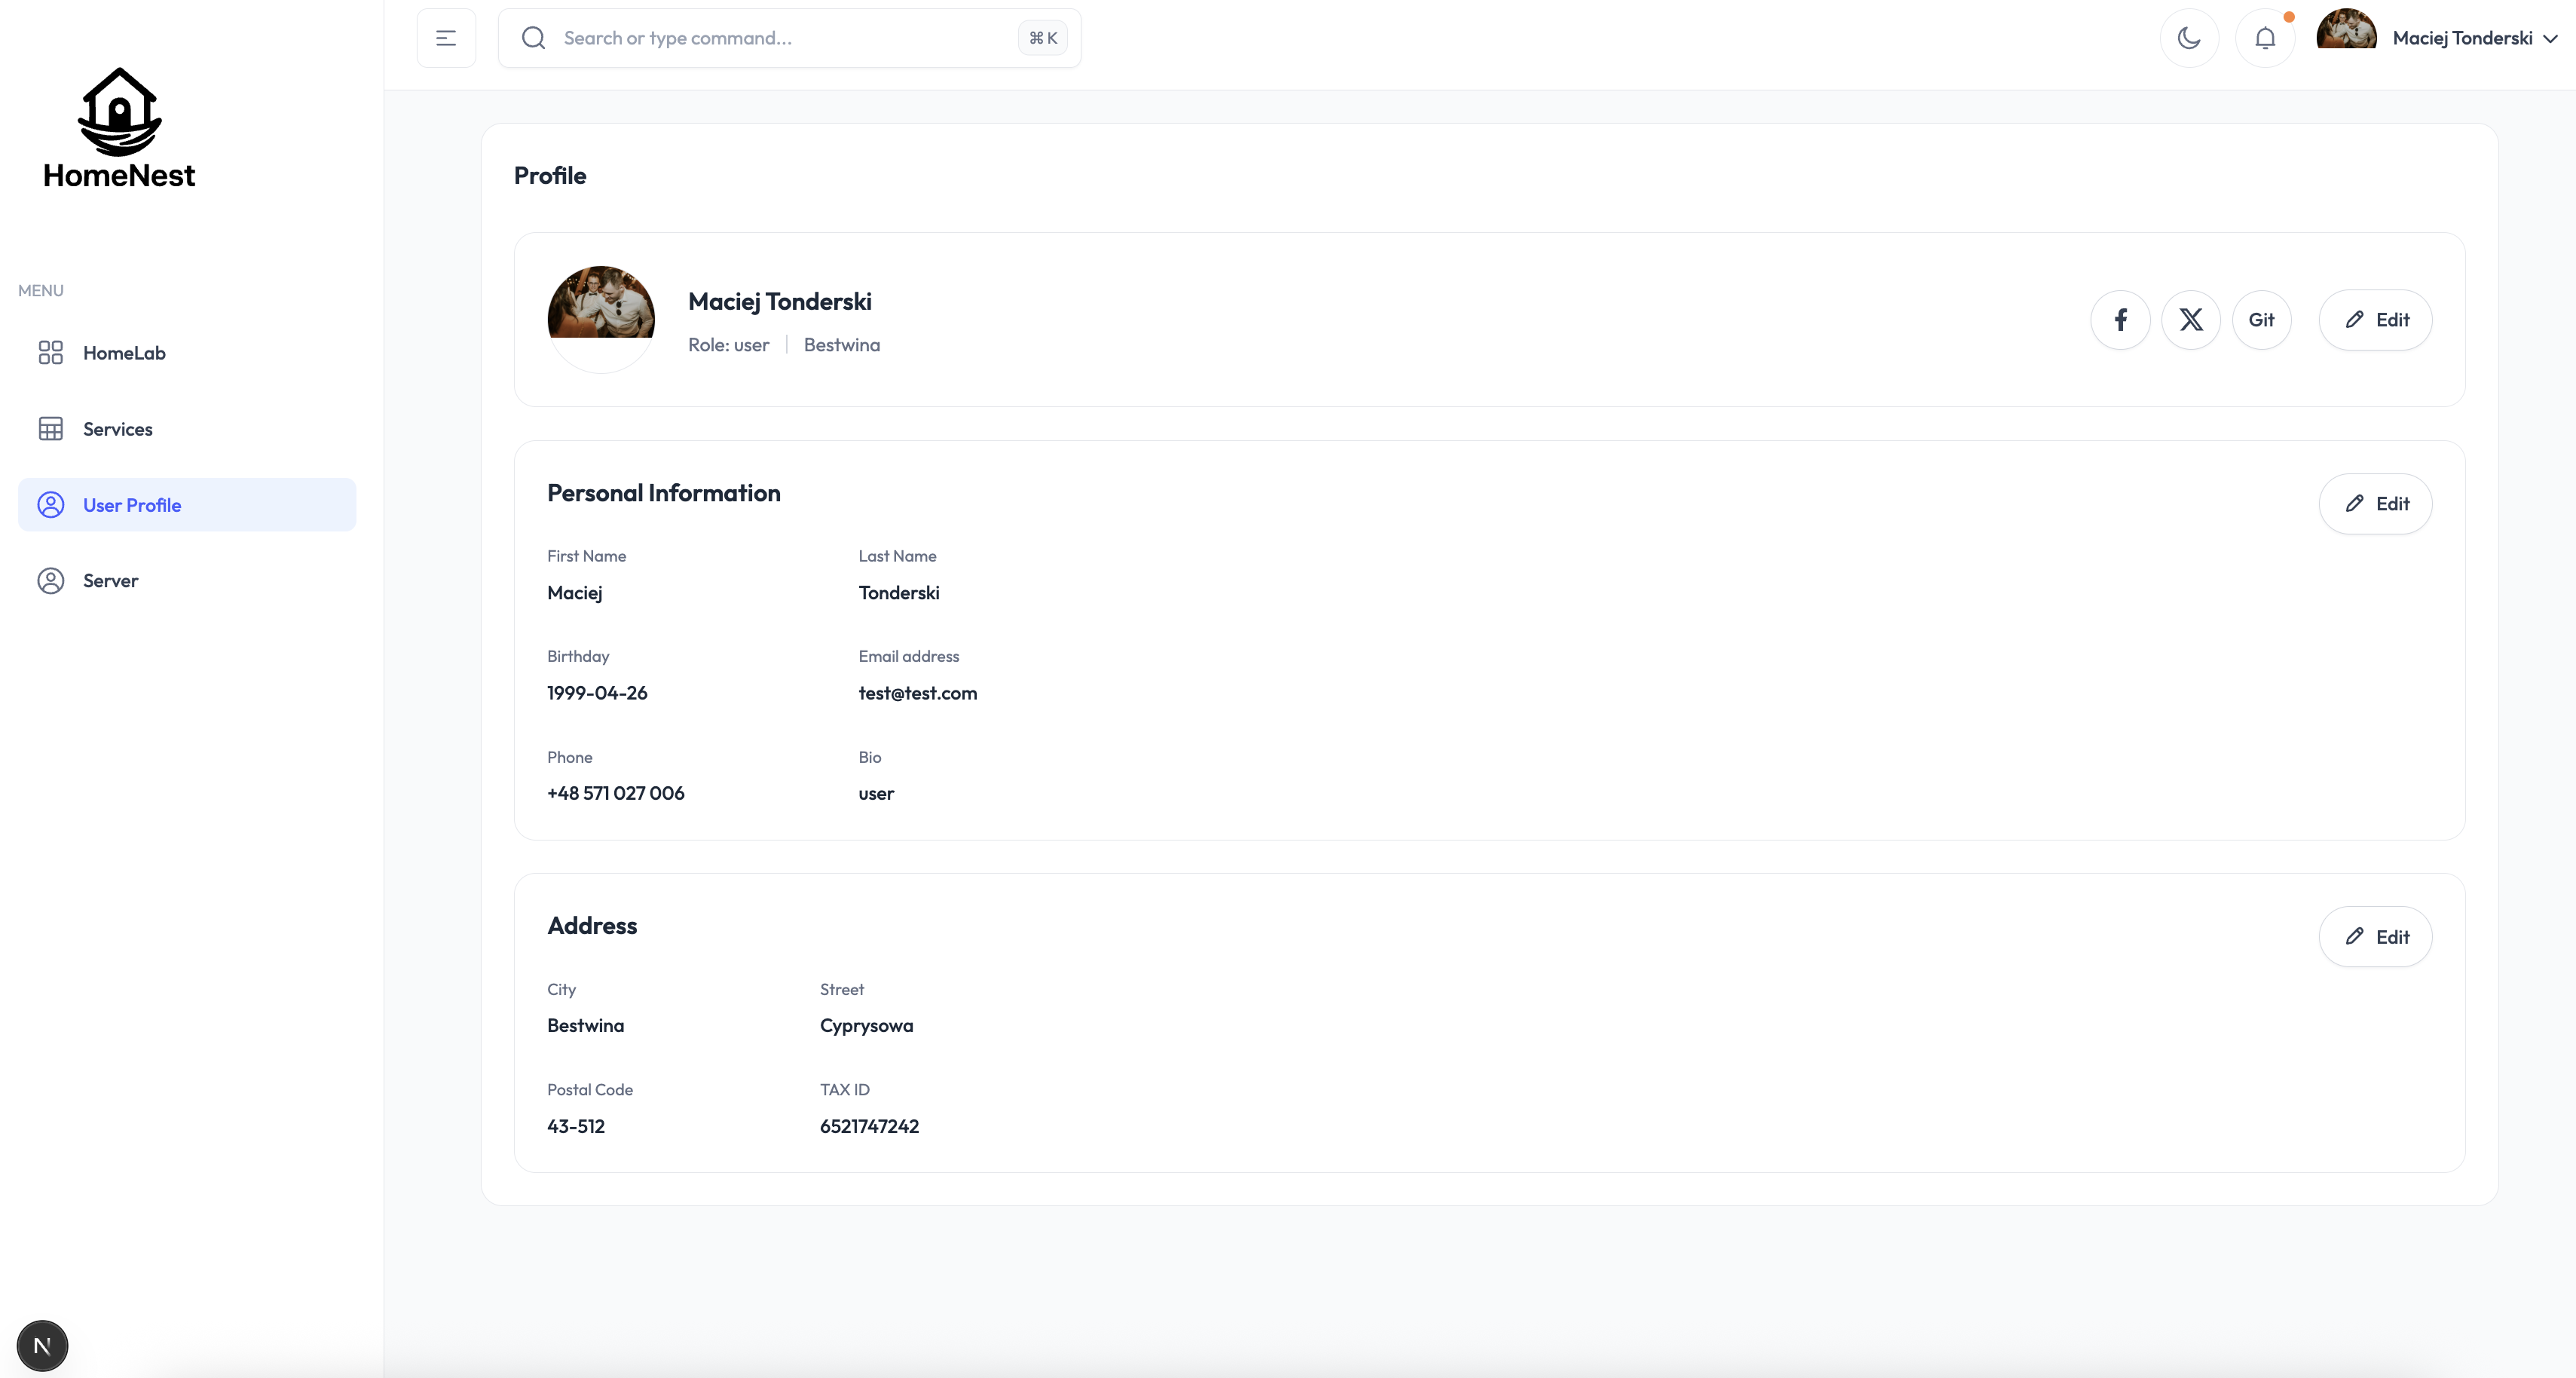
\includegraphics[width=1\textwidth]{./chapters/assets/profile_page.png}
  \caption{Podstrona aplikacji odpowiedzialna za wyświetlanie stanu obecnie uruchomionych aplikacji, pozwalająca na ich zarządzanie oraz przekierowująca użytkownika do serwisu.}
  \label{fig:ui_profile_page}
\end{figure}

\paragraph{Strona zarządzania serwerem}\mbox{}\\

Strona została zaprojektowana z myślą o administratorach systemu, zapewniając im intuicyjne komendy zarządzania serwerem oraz monitorowania jego wydajności i stabilności.

\begin{figure}[H]
  \centering
  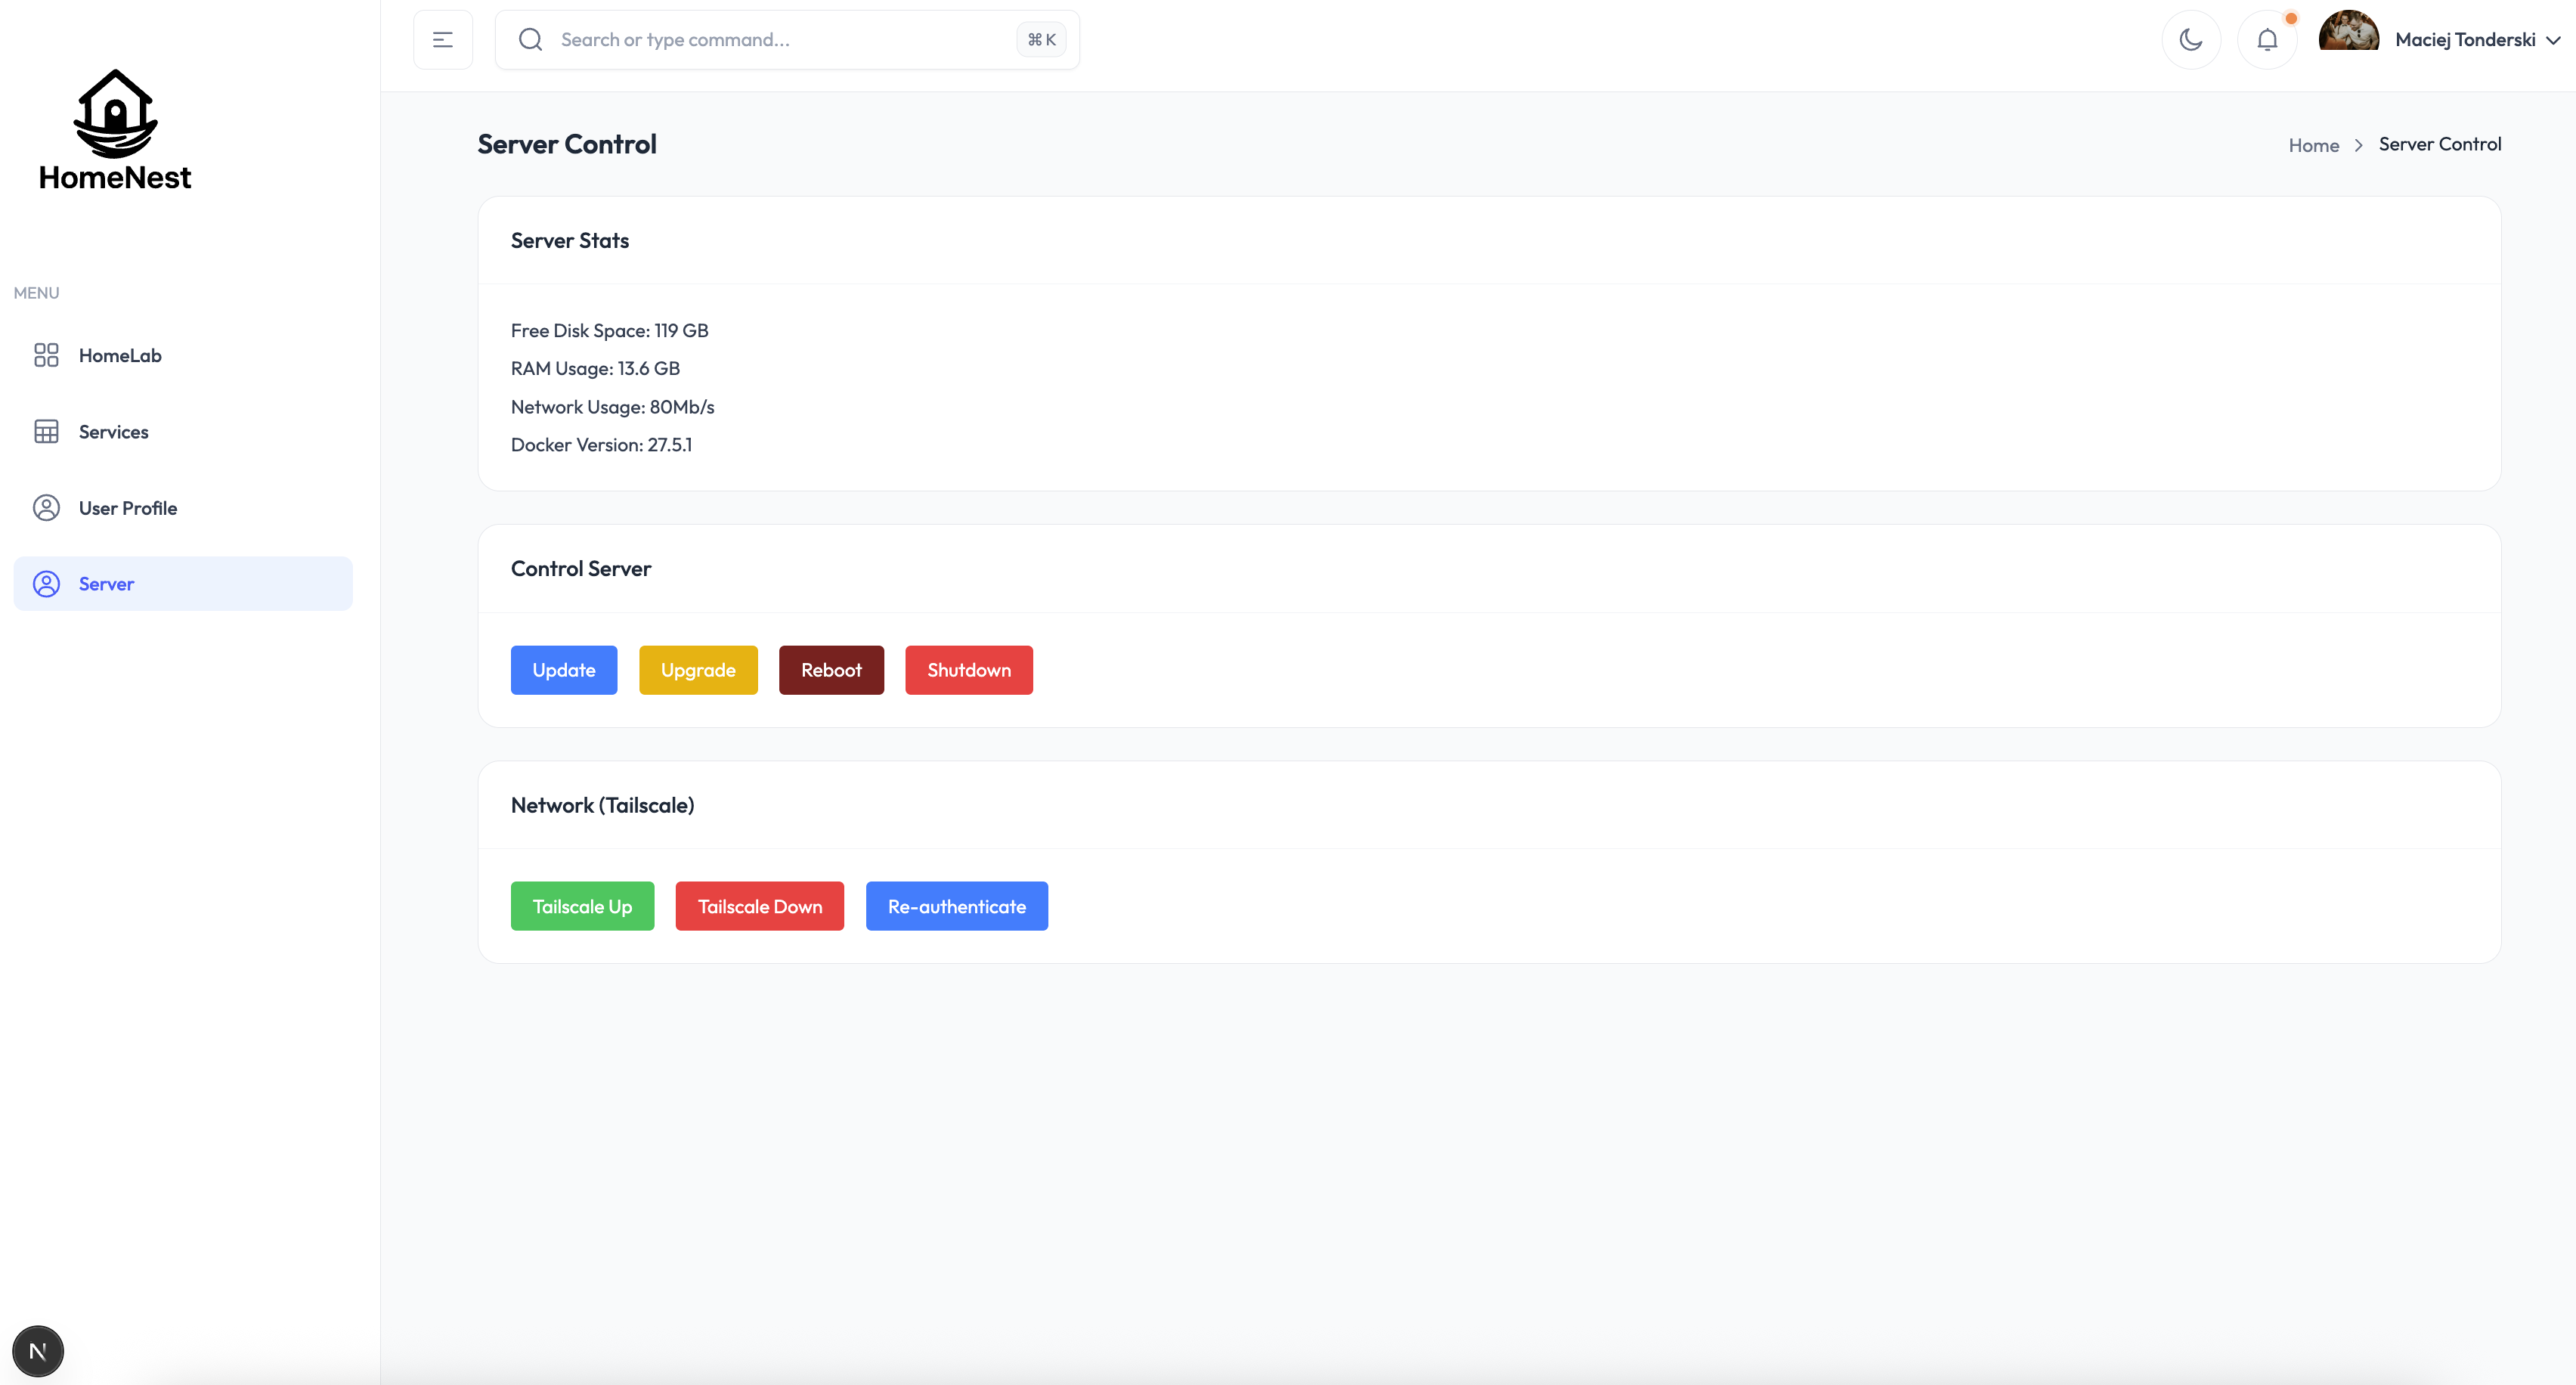
\includegraphics[width=1\textwidth]{./chapters/assets/server_page.png}
  \caption{Podstrona wyświetlająca informacje o stanie serwera, jego zasobach oraz umożliwiająca zarządzanie nimi.}
  \label{fig:ui_server_page}
\end{figure}
\noindent Strona przedstawiona na Rys. 4.7 zawiera następujące elementy:
\begin{itemize}
  \item \textbf{Panel Informacyjny -  Server Stats} - Zawiera informację na temat wykorzystanych zasobów serwera, takich jak CPU, RAM oraz przestrzeń dyskowa,
  \item \textbf{Panel Informacyjny -  Control Server} - Umożliwia użykotnikowi uruchomienie lub zatrzymanie serwera, a także zrestartowanie go. Użytkownik może również zaktualizować system operacyjny oraz zainstalować aktualizacje systemowe,
  \item \textbf{Panel Informacyjny -  Network (Tailscale\cite{Tailscale})} - Umożliwia użytkownikowi zarządzanie połączeniem z siecią Tailscale, w tym wyłączenie lub włączenie połączenia, przeprowadzenie procesu autoryzacji serwera.
\end{itemize}
\subsubsection{Kolorystyka i typografia}
Projekt interfejsu użytkownika aplikacji HomeNest wykorzystuje nowoczesną i spójną kolorystykę opartą na jasnym tle oraz delikatnych akcentach kolorystycznych. Dominującą barwą tła jest biel (\#ffffff), która nadaje przejrzystości oraz zapewnia wysoki kontrast względem elementów graficznych i tekstu.

Główne akcenty kolorystyczne w interfejsie stanowią odcienie niebieskiego (\#465fff, \#0ba5ec) wykorzystywane m.in. w wykresach, przyciskach akcji oraz wskaźnikach postępu. Barwy te pełnią funkcję informacyjną i nawigacyjną, kierując uwagę użytkownika na istotne elementy interfejsu. Kolorystyka została dodatkowo uzupełniona o neutralne odcienie szarości (\#667085, \#344054), które służą jako tło dla ikon, ramek i tekstów pomocniczych, umożliwiając ich subtelne wydzielenie bez nadmiernego rozpraszania użytkownika.

Zastosowana typografia oparta jest na nowoczesnym, bezszeryfowym kroju pisma, takim jak Outfit, który zapewnia wysoką czytelność niezależnie od rozdzielczości ekranu. Teksty nagłówków oraz wartości liczbowych zostały wyróżnione większym rozmiarem i wzmocnioną wagą fontu (font-medium, font-bold), co wspiera hierarchizację treści. Z kolei opisy pomocnicze oraz etykiety elementów interfejsu zostały zaprezentowane mniejszym rozmiarem i lżejszą barwą, dzięki czemu nie dominują wizualnie nad informacjami kluczowymi.

Zarówno kolorystyka, jak i typografia wspólnie tworzą minimalistyczny, intuicyjny interfejs, dostosowany do długotrwałego użytkowania oraz zgodny z aktualnymi standardami projektowania systemów zarządzania.

Aplikacja HomeNest wspiera również ciemny motyw interfejsu, co zostało zaprezentowane na rysunku poniżej. W tym trybie dominującym kolorem tła jest głęboka barwa granatowo-grafitowa (\#0c111d do \#1d2939), która w połączeniu z jasnymi akcentami (np. odcienie niebieskiego i bieli) zapewnia wysoki kontrast oraz elegancki, nowoczesny wygląd interfejsu.

Elementy interaktywne, jak przyciski czy wykresy, zachowują swoją kolorystykę, jednak są odpowiednio dostosowane do ciemnego tła - np. niebieskie słupki w wykresie API Calls, czy wskaźnik użycia dysku są wyraźnie widoczne również w warunkach ograniczonego oświetlenia.

Typografia w trybie ciemnym pozostaje spójna — fonty bezszeryfowe o wysokiej czytelności są renderowane z jasnymi odcieniami (\#ffffff, \#98a2b3), co sprzyja redukcji zmęczenia wzroku podczas pracy wieczorowej lub w zaciemnionym otoczeniu.

\paragraph{Korzyści wynikające z obsługi dwóch motywów kolorystycznych}\mbox{}\\

Zaprojektowanie interfejsu w dwóch wersjach — jasnej i ciemnej — jest coraz częściej stosowaną praktyką w nowoczesnych aplikacjach webowych i mobilnych. Taka decyzja projektowa niesie ze sobą szereg korzyści:
\begin{itemize}
  \item Dostosowanie do preferencji użytkownika
  Użytkownicy mają różne preferencje dotyczące komfortu pracy z interfejsem. Niektórzy wolą jasne motywy, które przypominają papier i są czytelne w jasnym otoczeniu. Inni preferują ciemne tryby, szczególnie wieczorem, gdy ograniczają zmęczenie wzroku i minimalizują emisję światła niebieskiego.
  \item Lepsze doświadczenie w różnych warunkach oświetleniowych
  Tryb jasny jest bardziej funkcjonalny w warunkach dziennego oświetlenia, natomiast tryb ciemny sprawdza się lepiej przy słabym świetle, np. podczas pracy nocą lub w pomieszczeniach bez dostępu do światła dziennego.
  \item Efektywność energetyczna (w przypadku ekranów OLED)
  W urządzeniach z ekranami OLED tryb ciemny może realnie wpłynąć na oszczędność energii, gdyż piksele wyświetlające kolor czarny są całkowicie wyłączone.
  \item Nowoczesny wygląd aplikacji
  Obsługa trybu ciemnego jest standardem UX w aplikacjach klasy premium i znacząco wpływa na odbiór estetyczny systemu, co może mieć pozytywne znaczenie marketingowe i wizerunkowe.
\end{itemize}


\subsection{Implementacja interfejsu użytkownika}

Interfejs użytkownika aplikacji HomeNest został zaimplementowany w oparciu o gotowy szablon \textbf{TailAdmin}\cite{TailAdmin}, który dostępny jest publicznie na licencji \textbf{MIT}. TailAdmin to nowoczesny szablon frontendowy oparty na technologii \textbf{React.js}, zbudowany przy użyciu frameworka \textbf{Next.js} oraz systemu stylów \textbf{Tailwind CSS}. Dzięki otwartej licencji możliwe było swobodne dostosowanie szablonu do potrzeb aplikacji oraz jego dalszy rozwój.

\subsubsection{Proces dostosowania szablonu}
W ramach prac wdrożeniowych wykonano następujące kroki:
\begin{enumerate}
    \item \textbf{Pobranie i uruchomienie szablonu} - Skonfigurowano środowisko developerskie oraz uruchomiono projekt TailAdmin w trybie deweloperskim.
    \item \textbf{Dostosowanie struktury aplikacji} - Zmodyfikowano układ nawigacji, menu, system routingu oraz strukturę stron zgodnie z architekturą systemu HomeNest.
    \item \textbf{Implementacja nowych widoków} - Zbudowano dedykowane widoki i komponenty, takie jak: panel główny, zarządzanie usługami, profil użytkownika oraz sekcja administracyjna serwera.
    \item \textbf{Integracja z API backendu} - Komponenty frontendowe zostały zintegrowane z API stworzonym w technologii Go. Dostosowanie szablonu TailAdmin do współpracy z tym API było zadaniem stosunkowo prostym, lecz wymagającym głębszej analizy w celu zoptymalizowania liczby zapytań wykonywanych do backendu oraz zapewnienia wydajnej komunikacji między warstwami systemu.
    \item \textbf{Wprowadzenie trybu ciemnego i jasnego} - Rozbudowano system motywów o możliwość przełączania pomiędzy trybem jasnym i ciemnym, z uwzględnieniem pełnej zgodności stylistycznej.
    \item \textbf{Refaktoryzacja i optymalizacja} - Usunięto zbędne fragmenty kodu, zoptymalizowano komponenty oraz uproszczono logikę interfejsu.
\end{enumerate}

\subsubsection{Zalety podejścia opartego na gotowym szablonie}
\begin{itemize}
    \item Znacząco skrócony czas implementacji frontendowej,
    \item Wysoka jakość kodu źródłowego i zgodność ze standardami branżowymi,
    \item Responsywne komponenty i nowoczesny design,
    \item Możliwość pełnej modyfikacji dzięki licencji MIT,
    \item Spójność wizualna i łatwość integracji z backendem.
\end{itemize}

\subsubsection{Wyzwania podczas adaptacji szablonu}
\begin{itemize}
    \item Konieczność analizy i zrozumienia istniejącej struktury projektu TailAdmin,
    \item Ręczne usuwanie niepotrzebnych widoków i kodu demonstracyjnego,
    \item Potrzeba dostosowania gotowych komponentów do wymagań aplikacji HomeNest,
    \item Zachowanie spójności wizualnej po wprowadzeniu nowych funkcjonalności.
\end{itemize}

Podsumowując, wykorzystanie TailAdmin jako szablonu bazowego pozwoliło na szybkie uruchomienie estetycznego i funkcjonalnego interfejsu użytkownika, a dzięki jego modularności i elastyczności możliwe było skuteczne dostosowanie go do specyfiki systemu HomeNest.


\section{Automatyzacja Konfiguracji i wdrozenie}

\subsection{Instalacja rozwiązania}
W ramach tworzenia rozwiązania powstał również program instalacyjny, który zostanie umieszczony na stronie internetowej rozwiązania umożliwiając pobranie przez zainteresowane korzystaniem z rozwiązania osoby.
\paragraph{Program instalacyjny}\mbox{}\\

W celu ułatwienia instalacji aplikacji na systemach użytkowników końcowych przygotowano dedykowany program instalacyjny napisany w języku Go. Aplikacja ta jest odpowiedzialna za:

\begin{itemize}
    \item Weryfikację obecności Dockera w systemie,
    \item Automatyczną instalację Dockera w systemach Linux (w pozostałych przypadkach użytkownik zostaje poinformowany o konieczności ręcznej instalacji),
    \item Pobranie najnowszej wersji aplikacji HomeNest z repozytorium GitHub,
    \item Rozpakowanie archiwum ZIP zawierającego aplikację do wskazanego katalogu,
    \item Nadanie odpowiednich uprawnień do uruchomienia aplikacji oraz jej uruchomienie.
\end{itemize}

Program wykorzystuje standardowe biblioteki Go do obsługi pobierania plików (\texttt{net/http}), rozpakowywania archiwów ZIP (\texttt{archive/zip}) oraz uruchamiania procesów lokalnych (\texttt{os/exec}). Dzięki temu działa w pełni samodzielnie, bez konieczności instalowania zewnętrznych zależności.

Logika działania programu obejmuje:
\begin{enumerate}
    \item Sprawdzenie czy polecenie \texttt{docker} znajduje się w ścieżce systemowej.
    \item Jeżeli Docker nie jest zainstalowany — uruchomienie skryptu instalacyjnego (tylko w systemach Linux).
    \item Pobranie pliku ZIP z GitHub Releases.
    \item Rozpakowanie pliku do katalogu roboczego.
    \item Uruchomienie pliku binarnego aplikacji.
\end{enumerate}

Instalator został zaprojektowany z myślą o prostocie użytkowania oraz możliwości łatwego wdrożenia aplikacji przez osoby nietechniczne. Wersje programu można przygotować na platformy Linux, Windows i macOS z wykorzystaniem narzędzia \texttt{GOOS/GOARCH}, umożliwiającego cross-kompilację.

\subsection{Integracja z narzędziami CI/CD}
\label{sec:integracja_ci_cd}

System HomeNest wykorzystuje mechanizmy CI/CD oparte na GitHub Actions\cite{Actions} w celu automatyzacji kluczowych procesów programistycznych — testowania, budowania, wersjonowania i publikacji aplikacji. Dzięki integracji z CI/CD możliwe jest zapewnienie ciągłości rozwoju i wysokiej jakości kodu bez potrzeby ręcznego wykonywania zadań wdrożeniowych.

\subsubsection{Schemat działania}

Po każdej zmianie wprowadzonej do głównej gałęzi \texttt{main}, automatycznie uruchamiane są dwa niezależne pipeline'y GitHub Actions:

\begin{enumerate}
    \item \textbf{Pipeline testujący} — weryfikuje jakość i poprawność kodu,
    \item \textbf{Pipeline release'owy} — buduje artefakty i tworzy release.
\end{enumerate}

\subsubsection{Pipeline testujący}

Pipeline testujący pełni funkcję strażnika jakości kodu. W jego ramach uruchamiane są:

\begin{itemize}
    \item \textbf{Linter} — analizuje kod źródłowy pod kątem zgodności ze standardami formatowania i stylu,
    \item \textbf{Testy jednostkowe backendu} — realizowane za pomocą \texttt{go test}.
\end{itemize}

Dzięki automatycznemu uruchamianiu testów możliwe jest wykrycie regresji i błędów już na etapie developmentu, zanim zostaną wprowadzone do środowiska produkcyjnego.

\subsubsection{Pipeline release'owy}

Po pozytywnym zakończeniu testów uruchamiany jest pipeline odpowiedzialny za zbudowanie artefaktów aplikacji oraz ich publikację jako nowego release'u na GitHubie. Proces ten jest realizowany przy pomocy pliku Makefile, który automatyzuje cały proces budowania i pakowania aplikacji. Makefile definiuje następujące cele:

\begin{itemize}
    \item \textbf{build-frontend} - instalacja zależności npm oraz zbudowanie aplikacji frontendowej; pliki wynikowe umieszczane są w katalogu \texttt{backend/static},
    \item \textbf{build-backend} - kompilacja aplikacji backendowej w Go z ustawieniem zmiennych środowiskowych \texttt{GOOS=linux} i \texttt{GOARCH=amd64}; wynikowy binarny plik jest zapisywany w katalogu \texttt{dist},
    \item \textbf{package} - kopiowanie plików frontendowych do katalogu dystrybucji oraz utworzenie archiwum \texttt{homelab.tar.gz},
    \item \textbf{clean} - usunięcie katalogów zbudowanych artefaktów i archiwum,
    \item \textbf{all} - domyślna akcja wykonująca czyszczenie, budowę frontendu i backendu oraz pakowanie.
\end{itemize}

Pipeline GitHub Actions wywołuje polecenie \texttt{make all}, co zapewnia spójność budowy na każdym etapie. Dzięki temu proces tworzenia release'u jest w pełni zautomatyzowany, powtarzalny i prosty do uruchomienia lokalnie.

\subsubsection{Przykładowy workflow GitHub Actions}

W poniższym przykładzie przedstawiono uproszczony workflow GitHub Actions, który wykorzystuje Makefile do budowania wszystkich komponentów systemu — frontend, backend oraz instalator:

\begin{lstlisting}
name: Release Build

on:
  push:
    branches: [main]

jobs:
  build:
    runs-on: ubuntu-latest

    steps:
    - name: Checkout repository
      uses: actions/checkout@v4

    - name: Set up Go
      uses: actions/setup-go@v4
      with:
        go-version: '1.21'

    - name: Set up Node.js
      uses: actions/setup-node@v3
      with:
        node-version: '20'

    - name: Install frontend dependencies
      run: cd frontend && npm ci

    - name: Build all components using Makefile
      run: make all

    - name: Build installer binaries
      run: |
        cd instalator
        make prepare
        make all

    - name: Archive release artifacts
      run: |
        mkdir release
        cp dist/homelab release/
        cp -r dist/static release/static
        cp instalator/build/* release/
        tar -czf release.tar.gz -C release .

    - name: Create GitHub Release
      uses: softprops/action-gh-release@v1
      with:
        tag_name: v${{ github.run_number }}
      env:
        GITHUB_TOKEN: ${{ secrets.GITHUB_TOKEN }}
      files: |
        release.tar.gz
\end{lstlisting}

\subsubsection{Strategia wersjonowania}

Każdy release oznaczany jest automatycznie na podstawie numeru buildu. W przyszłości możliwe będzie również wdrożenie semantycznego wersjonowania (SemVer) w oparciu o analizę commitów.

\subsubsection{Weryfikacja aktualności aplikacji}

W przyszłości system zostanie rozszerzony o mechanizm, który cyklicznie będzie odpytywał GitHub API w celu sprawdzenia dostępności nowego release'u. Porównując aktualnie zainstalowaną wersję z najnowszym tagiem, system będzie w stanie:

\begin{itemize}
    \item Powiadomić użytkownika o dostępnej aktualizacji,
    \item Wyświetlić changelog (opis zmian z release notes),
    \item Zaproponować pobranie i automatyczne wdrożenie nowej wersji.
\end{itemize}

Taka funkcjonalność przyczyni się do utrzymania systemu w najnowszej, stabilnej wersji bez potrzeby ręcznej ingerencji.

\subsubsection{Korzyści z automatyzacji CI/CD}

Integracja GitHub Actions pozwala na:

\begin{itemize}
    \item Skrócenie czasu wdrożeń,
    \item Unifikację procesu testowania i publikacji,
    \item Eliminację błędów ludzkich,
    \item Wzrost zaufania do jakości aplikacji,
    \item Łatwą replikację procesu na nowych środowiskach (np. staging, produkcja).
\end{itemize}

Dzięki powyższym cechom proces CI/CD jest nieodzownym elementem systemu HomeNest i fundamentem jego dalszego skalowania.